\documentclass[12pt,a4paper]{article}
\usepackage[utf8]{inputenc}
\usepackage{amsmath}
\usepackage{amsfonts}
\usepackage{amssymb}
\usepackage{graphicx}
\graphicspath{ {./img/} }
\usepackage{hyperref}
\usepackage{array}
\usepackage[table]{xcolor}
\usepackage{xcolor,colortbl}
\usepackage{multirow}
\usepackage[a4paper, total={6in, 8in}]{geometry}

\usepackage{titlesec}

\setcounter{secnumdepth}{4}

\titleformat{\paragraph}
{\normalfont\normalsize\bfseries}{\theparagraph}{1em}{}
\titlespacing*{\paragraph}
{0pt}{3.25ex plus 1ex minus .2ex}{1.5ex plus .2ex}

\author{Natale Guadagno, Paolo Patrone}
\title{Gestione dei Dati Persistenti - TecStore}
\renewcommand{\contentsname}{Contenuti}

\usepackage{hyperref}
\hypersetup{
    colorlinks,
        citecolor=blue,
    filecolor=blue,
    linkcolor=blue,
    urlcolor=blue,
    linktocpage
}

\begin{document}

\maketitle
\newpage
\tableofcontents
\newpage
\newgeometry{top=0.5in,bottom=0.5in,right=0.5in,left=0.5in}
\section*{Partecipanti}
\begin{center}
\begin{tabular} {|c|c|}
\hline
\textbf{Nome} & \textbf{Matricola} \\
\hline
Guadagno Natale & 0512106546 \\
Patrone Paolo & 0512106153 \\
\hline
\end{tabular}
\end{center}
\newpage

\section{Class diagram}
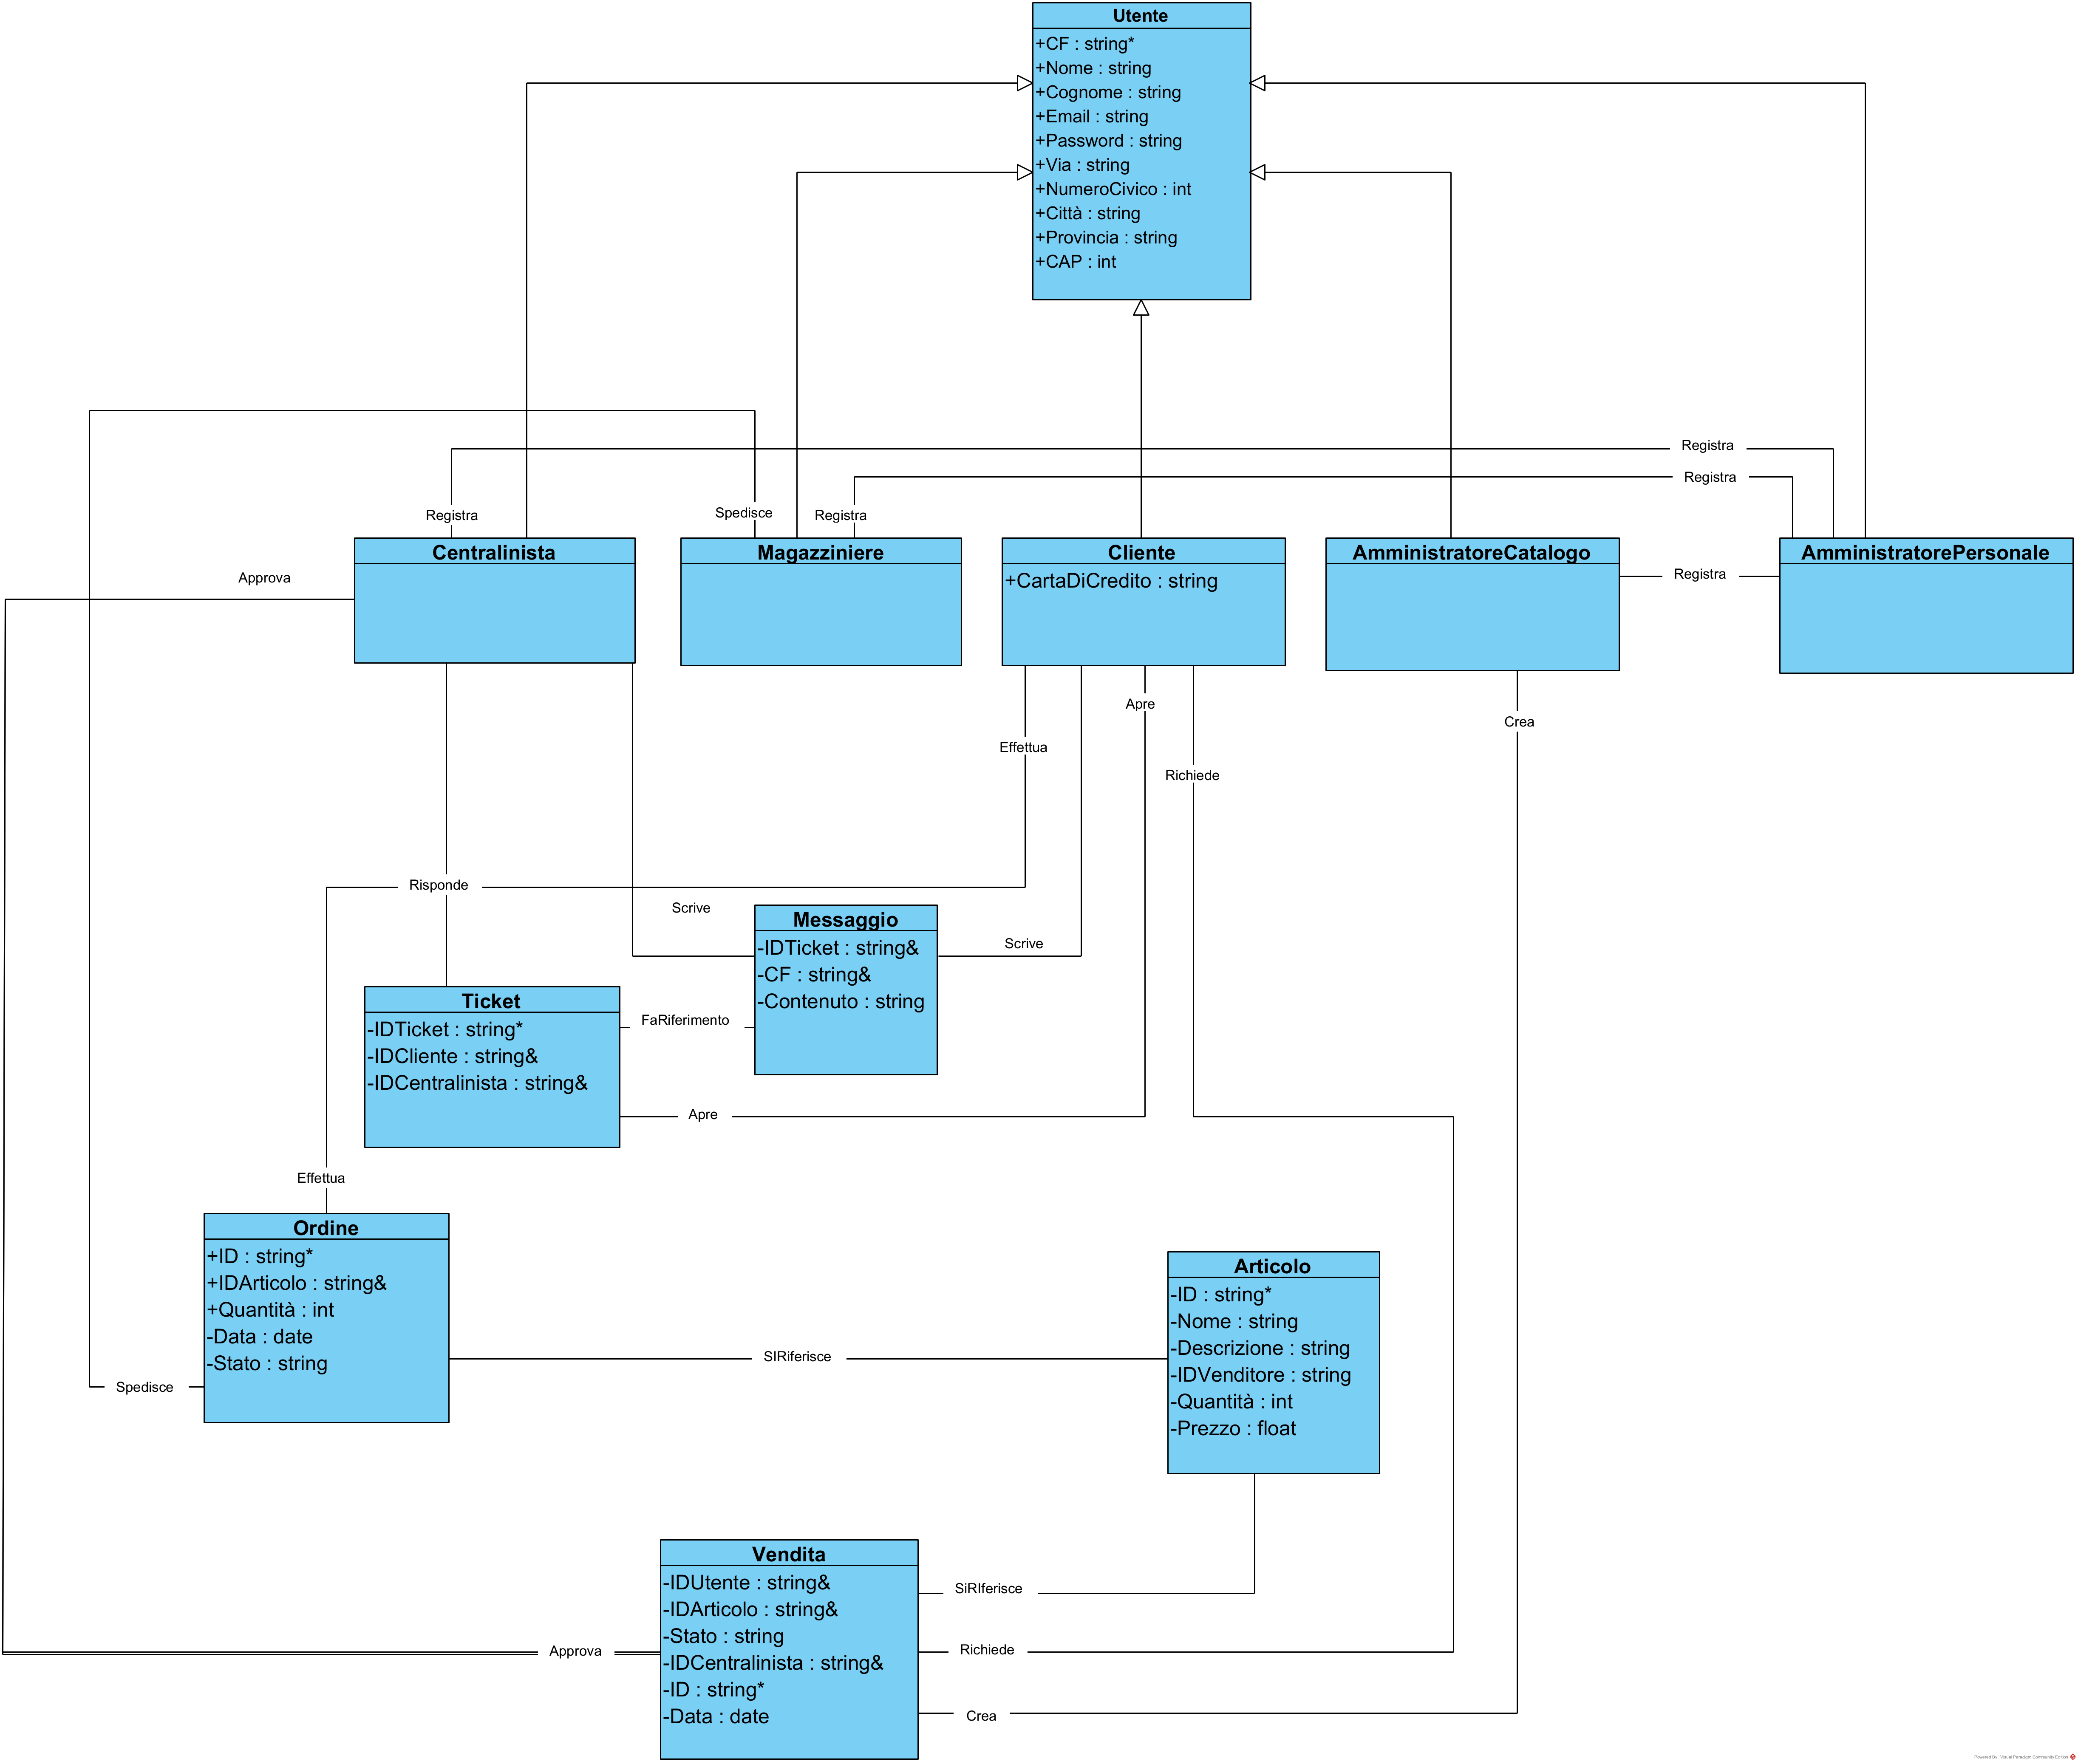
\includegraphics[width=\textwidth]{../RAD/img/DiagrammaDiClasse}

\subsection{Mapping del database}
\textbf{articolo}(\underline{\textbf{ID}}, Nome, Descrizione, IDVenditore $\uparrow$, Quantita, Prezzo, Stato, IDCentralinista $\uparrow$, data, rimborsabile) \\
\textbf{Carrello}(IDCliente $\uparrow$, IDArticolo $\uparrow$, Quantita) \\
\textbf{Foto}(\underline{\textbf{ID}}, IDArticolo $\uparrow$, Foto) \\
\textbf{Messaggio}(IDTicket $\uparrow$, CF $\uparrow$, Contenuto, Data) \\
\textbf{Ordine}(\underline{\textbf{ID}}, IDCliente $\uparrow$, IDArticolo $\uparrow$, Quantita, Stato, Data, CodiceTracciamento)\\
\textbf{Ticket}(\underline{\textbf{IDTicket}}, IDCliente $\uparrow$, Tipologia, Stato, DataCreazione) \\
\textbf{Utente}(\underline{\textbf{CF}}, Nome, Cognome, Email, Password, Via, NumeroCivico, Citta, Provincia, CAP, Tipologia, CartaDiCredito)

\section{Struttura delle tabelle}

\subsection{Utente}
\begin{center}
\begin{tabular}{|l|l|l|l|l|}
\hline
\rowcolor[HTML]{C0C0C0} 
\textbf{Nome} & \textbf{Tipo} & \textbf{Vincoli} & \textbf{Chiavi} & \textbf{Default}  \\ \hline
CF & CHAR(16) & NOT NULL & PRIMARY KEY &  \\ \hline
Nome & VARCHAR(45) & NOT NULL & & \\ \hline
Cognome & VARCHAR(45) & NOT NULL & & \\ \hline
Email & VARCHAR(45) & NOT NULL & & \\ \hline
Password & VARCHAR(60) & NOT NULL & & \\ \hline
Via & VARCHAR(60) & NOT NULL & & \\ \hline
NumeroCivico & VARCHAR(8) & NOT NULL & & \\ \hline
Citta & VARCHAR(45) & NOT NULL & & \\ \hline
Provincia & CHAR(2) & NOT NULL & & \\ \hline
CAP & INT(5) & NOT NULL && \\ \hline
Tipologia & INT(1) & NOT NULL && \\ \hline
CartaDiCredito & CHAR(16) &&& \\ \hline
\end{tabular}
\end{center}

\subsubsection{Articolo}

\begin{center}
\begin{tabular}{|l|l|l|l|l|}
\hline
\rowcolor[HTML]{C0C0C0} 
\textbf{Nome} & \textbf{Tipo} & \textbf{Vincoli} & \textbf{Chiavi} & \textbf{Default}  \\ \hline
ID & VARCHAR(45) & NOT NULL & PRIMARY KEY & UUID() \\ \hline
Nome & VARCHAR(45) & NOT NULL & & \\ \hline
Descrizione & VARCHAR(512) & NOT NULL & & \\ \hline
IDVenditore & CHAR(16) & NOT NULL & FOREIGN KEY (Utente)& \\ \hline
Quantita & INT(3) & NOT NULL & & \\ \hline
Prezzo & FLOAT(5,2) & NOT NULL & & \\ \hline
Stato & VARCHAR(45) & NOT NULL & & \\ \hline
IDCentralinista & CHAR(16) & & FOREIGN KEY (Utente) & NULL \\ \hline
Data & TIMESTAMP & NOT NULL & TIMESTAMP() & \\ \hline
Rimborsabile & TINYINT(4) & NOT NULL & & \\ \hline
\end{tabular}
\end{center}

\subsubsection{Foto}
\begin{center}
\begin{tabular}{|l|l|l|l|l|}
\hline
\rowcolor[HTML]{C0C0C0} 
\textbf{Nome} & \textbf{Tipo} & \textbf{Vincoli} & \textbf{Chiavi} & \textbf{Default}  \\ \hline
ID & VARCHAR(45) & NOT NULL & PRIMARY KEY & UUID() \\ \hline
IDArticolo & VARCHAR(45) & & FOREIGN KEY (Articolo)& \\ \hline
Foto & MEDIUMBLOBL & & & \\ \hline
\end{tabular}
\end{center}

\subsubsection{Carrello}
\begin{center}
\begin{tabular}{|l|l|l|l|l|}
\hline
\rowcolor[HTML]{C0C0C0} 
\textbf{Nome} & \textbf{Tipo} & \textbf{Vincoli} & \textbf{Chiavi} & \textbf{Default}  \\ \hline
IDArticolo & VARCHAR(45) & NOT NULL & PRIMARY KEY, FOREIGN KEY(Articolo) & \\ \hline
IDVenditore & CHAR(16) & NOT NULL & PRIMARY KEY, FOREIGN KEY (Utente)& \\ \hline
Quantita & INT(11) & NOT NULL & & \\ \hline
\end{tabular}
\end{center}

\newpage

\subsection{Ticket}
\begin{center}
\begin{tabular}{|l|l|l|l|l|}
\hline
\rowcolor[HTML]{C0C0C0} 
\textbf{Nome} & \textbf{Tipo} & \textbf{Vincoli} & \textbf{Chiavi} & \textbf{Default}  \\ \hline
IDTicket & VARCHAR(45) & NOT NULL & FOREIGN KEY(Ticket) & \\ \hline
IDCliente & CHAR(16) & NOT NULL & FOREIGN KEY (Utente)& \\ \hline
Tipologia & VARCHAR(45) & & & \\ \hline
Stato & VARCHAR(45) & NOT NULL & & \\ \hline
DataCreazione & TIMESTAMP & NOT NULL & & TIMESTAMP() \\ \hline
\end{tabular}
\end{center}


\subsection{Messaggio}
\begin{center}
\begin{tabular}{|l|l|l|l|l|}
\hline
\rowcolor[HTML]{C0C0C0} 
\textbf{Nome} & \textbf{Tipo} & \textbf{Vincoli} & \textbf{Chiavi} & \textbf{Default}  \\ \hline
IDTicket & VARCHAR(45) & NOT NULL & FOREIGN KEY(Ticket) & \\ \hline
CF & CHAR(16) & NOT NULL & FOREIGN KEY (Utente)& \\ \hline
Contenuto & VARCHAR(512) & NOT NULL & & \\ \hline
Data & TIMESTAMP & NOT NULL & & TIMESTAMP() \\ \hline
\end{tabular}
\end{center}

\subsection{Ordine}
\begin{center}
\begin{tabular}{|l|l|l|l|l|}
\hline
\rowcolor[HTML]{C0C0C0} 
\textbf{Nome} & \textbf{Tipo} & \textbf{Vincoli} & \textbf{Chiavi} & \textbf{Default}  \\ \hline
ID & VARCHAR(45) & NOT NULL & PRIMARY KEY & UUID() \\ \hline
IDCliente & CHAR(16) & NOT NULL & FOREIGN KEY (Utente)& \\ \hline
IDArticolo & VARCHAR(45) & & FOREIGN KEY (Articolo)& \\ \hline
Quantita & INT(3) & NOT NULL & & \\ \hline
Stato & VARCHAR(45) & NOT NULL & & \\ \hline
Data & TIMESTAMP & NOT NULL & & TIMESTAMP() \\ \hline
CodiceTracciamento & VARCHAR(45) & & \\ \hline
\end{tabular}
\end{center}


\end{document}